\section{Método da Iteração QR}

\begin{itemize}

\item É um método de transformação.

\item Os métodos de transformação utilizam as propriedades básicas dos autovalores na matriz

\begin{equation}
 \label{cap5:sec5:eq1}
 \matriz{X} = [\vetorl{x_1} \vetorl{x_2} \ldots \vetorl{x_n} ]
\end{equation}

\noindent
cujas colunas são os $ N $ autovetores da matriz $ \matriz{A} $ do problema de autovalores

\begin{equation}
 \label{cap5:sec5:eq2}
 \matriz{A} \vetorl{x_i} = \lambda_i \vetorl{x_i}
\end{equation}

\end{itemize}

A matriz $ \matriz{X} $ diagonaliza a matriz $ \matriz{A} $, ou seja,

\begin{equation}
 \label{cap5:sec5:eq3}
 \matriz{X^T} \matriz{A} \matriz{X} = \matriz{\Lambda}
\end{equation}

\noindent
onde

\begin{equation}
 \label{cap5:sec5:eq4}
 \Lambda = diag \, (\lambda_1, \, \lambda_2, \, \ldots, \, \lambda_n)
\end{equation}

O princípio básico dos métodos de transformação é construir $ \matriz{X} $ de forma iterativa aplicando transformações de similaridade com o objetivo de diagonalizar $ \matriz{A} $.

\begin{equation}
 \label{cap5:sec5:eq5}
 \begin{array}{cl}
  \matriz{A_1} & = \matriz{A}\\
  \matriz{A_2} & = \matriz{P_1^T} \matriz{A_1} \matriz{P_1}\\
  \matriz{A_3} & = \matriz{P_2^T} \matriz{A_2} \matriz{P_2} = \matriz{P_2^T} \matriz{P_1^T} \matriz{A_1} \matriz{P_1} \matriz{P_2}\\
  \vdots &\\
  \matriz{A_{k+1}} & = \matriz{P_k^T} \matriz{A_k} \matriz{P_k} = \matriz{P_k^T} \matriz{P_{k-1}^T} \ldots \matriz{P_2^T} \matriz{P_1^T} \matriz{A} \matriz{P_1} \matriz{P_2} \ldots \matriz{P_{k-1}} \matriz{P_k}
 \end{array} 
\end{equation}

Quando $ k \rightarrow \infty $,

\begin{equation}
 \label{cap5:sec5:eq6}
 \matriz{A_{k+1}} \rightarrow \matriz{\Lambda}
\end{equation}

\subsection{Método de Jacobi}

\begin{equation}
 \label{cap5:sec5:eq7}
 \matriz{A_{k+1}} = \matriz{P_k^T} \matriz{A_k} \matriz{P_k}
\end{equation}

\noindent
onde $ \matriz{P_k} $ é uma matriz ortonormal

\begin{equation}
 \label{cap5:sec5:eq8}
 \matriz{P_k^T} \matriz{P_k} = \matriz{I}
\end{equation}

No método de Jacobi a matriz $ \matriz{P_k} $ é uma matriz de rotação selecionada de forma a zerar um elemento fora da diagonal de $ \matriz{A_k} $.

Para zerar o elemento $ (i,j) $.

\begin{equation}
 \begin{array}{c}

  \matriz{P_k}
  =
  \left[
  \begin{array}{cccccccccccc}
   1 &         &    &                      &   &         &   &                       &   &        &   &\\
     & \ddots  &    &                      &   &         &   &                       &   &        &   &\\
     &         & 1  &                      &   &         &   &                       &   &        &   &\\
     &         &    & \mbox{cos} \, \theta &   &         &   & -\mbox{sen} \, \theta &   &        &   &\\
     &         &    &                      & 1 &         &   &                       &   &        &   &\\
     &         &    &                      &   & \ddots  &   &                       &   &        &   &\\
     &         &    &                      &   &         & 1 &                       &   &        &   &\\
     &         &    & \mbox{sen} \, \theta &   &         &   & \mbox{cos} \, \theta  &   &        &   &\\
     &         &    &                      &   &         &   &                       & 1 &        &   &\\
     &         &    &                      &   &         &   &                       &   & \ddots &   &\\
     &         &    &                      &   &         &   &                       &   &        & 1 &\\
  \end{array}
  \right]
  \begin{array}{c}
    \\
    \\
    \\
   i\\
    \\
    \\
    \\
   j\\
    \\
    \\
    \\
  \end{array}
  \\
  i \hspace*{3cm} j

 \end{array}
\end{equation}

\noindent
onde $ \theta $ é o ângulo tal que

\begin{equation}
 \left\{
 \begin{array}{lll}
  \tan \, (2 \, \theta)   & = \displaystyle \frac{2 \, a_{ij}^{(k)}}{a_{ii}^{(k)} - a_{jj}^{(k)}} & \mbox{p/} \, a_{ii}^{(k)} \neq a_{jj}^{(k)} \\
  \theta = \displaystyle \frac{\pi}{4}, & 							                  & \mbox{p/} \, a_{ii}^{(k)} = a_{jj}^{(k)}
 \end{array}
 \right.
\end{equation}

\begin{itemize}

\item Varreduras por linha ou por coluna $ n \, (n - 1) $ matrizes $ \matriz{P} $.

\item Elementos que foram zerados podem deixar de ser zero durante o processo.

\item Várias varreduras são necessárias.

\end{itemize}

\[
\begin{array}{l}
 A_{ij} = A_{ji} = 0 = P_{ik}^T \, A_{kl} \, P_{lj} = P_{ji} \, A_{kl} \, P_{lj} \Rightarrow \\ \vspace*{0.3cm}
 0 = \displaystyle \sum_{l=1}^n \, \left[ \sum_{k=1}^n \, P_{ki} \, A_{kl} \right] \, P_{lj} = \sum_{l=1}^n \, \left[ P_{ii} \, A_{il} + P_{ji} \, A_{jl} \right] P_{lj} = \\ \vspace*{0.3cm}
 = P_{ii} \, A_{ii} \, P_{ij} + P_{ii} \, A_{ij} \, P_{jj} + P_{ji} \, A_{ji} \, P_{ij} + P_{ji} \, A_{jj} \, P_{jj} \\ \vspace*{0.3cm}
 = \cos \theta \, \, A_{ii} \, (-\mbox{sen} \, \theta) + \cos \theta \, \, A_{ij} \, \cos \theta + \mbox{sen} \, \, \theta \, A_{ji} \, (-\mbox{sen} \, \theta) + \mbox{sen} \, \theta \, \, A_{jj} \, \cos \, \theta\\ \vspace*{0.3cm}
 = -\mbox{sen} \, \theta \, \, \cos \theta \, (A_{ii} - A_{jj}) + (\cos^2 \theta - \mbox{sen}^2 \, \theta) \, A_{ij} \Rightarrow \\ \vspace*{0.3cm}
 \Rightarrow \mbox{sen} \, \theta \, \cos \theta \, (A_{ii} - A_{jj}) = (\cos^2 \theta - \mbox{sen}^2 \, \theta) \, A_{ij}\\ \vspace*{0.3cm}
 \displaystyle \frac{\mbox{sen} \, 2 \, \theta}{\cos 2 \, \theta} = \frac{2 \, A_{ij}}{A_{ii} - A_{jj}}\\ \vspace*{0.3cm}
 \mbox{ \framebox{ $ \tan \, (2 \, \theta) = \displaystyle \frac{2 \, A_{ij}}{A_{ii} - A_{jj}} $ } }
\end{array}
\]

\begin{figure}[htb]
 \centering
 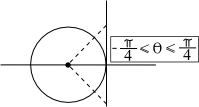
\includegraphics[scale=1.0]{capitulos/capitulo5/figuras/met_iter_qr1.png}
 \caption{?}
 \label{fig:met_iter_qr1}
\end{figure}

A multiplicação em \ref{cap5:sec5:eq7} afeta apenas os termos da matriz $ A_{k} $ nas linhas $ i $ e $ j $ e nas colunas $ i $ e $ j $. Assim,

\begin{equation}
 \label{cap5:sec5:eq10}
 \begin{array}{cl}
  (A_{ii})_{k+1} & = (A_{ii} \, \cos^2 \theta + 2 \, A_{ij} \, \cos \theta \, \mbox{sen} \, \theta + A_{jj} \, \mbox{sen}^2 \, \theta)_k \\
  (A_{jj})_{k+1} & = (A_{ii} \, \mbox{sen}^2 \, \theta - 2 \, A_{ij} \, \cos \theta \, \mbox{sen} \, \theta + A_{jj} \, \cos^2 \theta)_k \\
  (A_{ij})_{k+1} & = (A_{ji})_{k+1} = 0 \\
  (A_{li})_{k+1} & = (A_{il})_{k+1} = (A_{li} \, \cos \theta + A_{lj} \, \mbox{sen} \, \theta)_k \\
  (A_{lj})_{k+1} & = (A_{jl})_{k+1} = (-A_{li} \, \, \mbox{sen} \, \theta + A_{lj} \, \cos \theta)_k
 \end{array}
\end{equation}

\subsection{Método QR}

O passo básico do método é decompor a matriz $ \matriz{A} $ na forma

\begin{equation}
 \label{cap5:sec5:eq11}
 \matriz{A} = \matriz{Q} \matriz{R}
\end{equation}

\noindent
onde $ \matriz{Q} $ é uma matriz ortogonal e $ \matriz{R} $ é uma matriz triangular superior.

Depois, formamos a matriz $ \matriz{R} \matriz{Q} $

\begin{equation}
 \label{cap5:sec5:eq12}
 \matriz{R} \matriz{Q} = \matriz{Q^T} \matriz{A} \matriz{Q}
\end{equation}

\[
 \begin{array}{l}
  \matriz{A} = \matriz{Q} \matriz{R} \Rightarrow \matriz{Q^T} \matriz{A} \matriz{Q} = \underbrace{\matriz{Q^T} \matriz{Q}}_{\matriz{I}} \matriz{R} \matriz{Q} = \matriz{R} \matriz{Q}
 \end{array}
\]

OBS: O produto $ \matriz{R} \matriz{Q} $ corresponde a uma transformação de similaridade em $ \matriz{A} $.\\

Como obtemos a decomposição $ \matriz{Q} \matriz{R} $?

Aplicamos matrizes de rotação de Jacobi para transformar $ \matriz{A} $ em $ \matriz{R} $. Assim

\begin{equation}
 \label{cap5:sec5:eq13}
 \begin{array}{l}
  \underbrace{P_{n,\,n-1}^T \, \ldots \matriz{P_{3,1}^T} \matriz{P_{2,1}^T}}_{\matriz{Q^T}} \matriz{A} = \matriz{R}
 \end{array}
%  \qquad \qquad
%  \begin{array}{c}
% 
%   P^T_{j\,i}
%   =
%   \left[
%   \begin{array}{ccccccccc}
%    1 &         &                       &   &         &   &                       &   &\\
%      &         & \mbox{cos} \, \theta  &   &         &   & \mbox{sen} \, \theta  &   &\\
%      &         &                       & 1 &         &   &                       &   &\\
%      &         &                       &   & \ddots  &   &                       &   &\\
%      &         &                       &   &         & 1 &                       &   &\\
%      &         & -\mbox{sen} \, \theta &   &         &   & \mbox{cos} \, \theta  &   &\\
%      &         &                       &   &         &   &                       & 1 &\\
%   \end{array}
%   \right]
%   \begin{array}{c}
%     \\
%    i\\
%     \\
%     \\
%     \\
%    j\\
%     \\
%   \end{array}
%   \\
%   i \hspace*{3cm} j
% 
%  \end{array}
\end{equation}

Processo iterativo $ \matriz{A_1} = \matriz{A} $

\begin{equation}
 \label{cap5:sec5:eq14}
 \begin{array}{rcl}
  & \mbox{ \footnotesize{(\ref{cap5:sec5:eq13})} } & \\
  \matriz{A_k} & = & \matriz{Q_k} \matriz{R_k}
 \end{array}
\end{equation}

\begin{equation}
 \label{cap5:sec5:eq15}
 \matriz{A_{k+1}} = \matriz{R'_?} \matriz{Q_?}
\end{equation}

\[
 \left.
 \begin{array}{l}
  \matriz{A_{k+1}} \rightarrow \matriz{\Lambda} \\
  Q_1 \, \ldots \, \, Q_{k-1} \, Q_k \rightarrow \matriz{X}
 \end{array}
 \right\}
 \, k \rightarrow \infty
\]

Se aplicarmos matrizes de rotação de Jacobi para transformar $ A $ em $ R $ (triangular superior).

Com $ i > j $ :

\[
 \begin{array}{ll}
  R_{ij} & = 0 = P_{ik}^T \, A_{kj} = P_{ki} \, A_{kj}\\
         & = P_{ji} \, A_{jj} + P_{ii} \, A_{ij}\\ \vspace*{0.3cm}
         & = -\mbox{sen} \, \theta \, A_{jj} + cos \, \theta \, A_{ij} \Rightarrow \mbox{\framebox{ $ \tan \, \theta = \displaystyle \frac{A_{ij}}{A_{jj}} $ }}
 \end{array}
%  \qquad \qquad
%  \begin{array}{c}
% 
%   \begin{array}{c}
%     \\
%    j\\
%     \\
%    i\\
%     \\
%   \end{array}
%   \left[
%   \begin{array}{ccccccccc}
%      &         &                       &   &         &   &                       &   &\\
%      &         & \mbox{cos} \, \theta  &   &         &   & -\mbox{sen} \, \theta &   &\\
%      &         &                       &   & \ddots  &   &                       &   &\\
%      &         & \mbox{sen} \, \theta  &   &         &   & \mbox{cos} \, \theta  &   &\\
%      &         &                       &   &         &   &                       &   &\\
%   \end{array}
%   \right]
%   \\
%   j \hspace*{3cm} i
% 
%  \end{array}
\]

\noindent
ou

\[
 \begin{array}{ll}
              & \mbox{sen} \, \theta \, A_{jj} = \cos \, \theta \, A_{ij} \Rightarrow \mbox{sen}^2 \, \theta \, A_{ji}^2 - \cos^2 \, \theta \, A_{ij}^2 = 0 \\ \vspace*{0.3cm}
  \Rightarrow & \mbox{sen}^2 \, \theta \, A_{jj}^2 - (1 - \mbox{sen}^2 \, \theta) \, A_{ij}^2 = 0 \Rightarrow \\
  \Rightarrow & \mbox{sen}^2 \, \theta \, (A_{jj}^2 + A_{ij}^2) = A_{ij}^2 \Rightarrow \mbox{\framebox{ $ \mbox{sen} \, \theta = \displaystyle \frac{A_{ij}}{\sqrt{A_{ij}^2 + A_{jj}^2}} $ }}\\ \\
              & \mbox{\framebox{ $ \cos \, \theta = \displaystyle \frac{A_{jj}}{\sqrt{A_{ij}^2 + A_{jj}^2}} $ }}
 \end{array}
\]
